\documentclass[10pt]{article}
\usepackage[letterpaper,landscape,margin=0.65in]{geometry}
\usepackage{graphicx}
\usepackage{booktabs}
\usepackage[T1]{fontenc}
\usepackage{hyperref}
\hypersetup{pdftitle={FROB C5 finite-field trace proof audit},
  pdfsubject={EXP-FROB-91ee9c; finite-field trace core proved; run bridges open}}
\setlength{\parindent}{0pt}
\setlength{\parskip}{0.45em}
\title{FROB C5 finite-field trace proof audit}
\author{Validation audit, 22 October 2026}
\date{}
\begin{document}
\maketitle
\vspace{-2em}

\textbf{Scope.} Frozen \texttt{EXP-FROB-91ee9c} control C5;
Lean source commit \texttt{0600270bcf4a49edfb65d0fe838ab5fa4442216c}.
This is a mathematical proof slice, not a new experiment or performance result.

\begin{center}
\begin{tabular}{lll}
\toprule
Lean conclusion & Exact scope & Beyond this theorem \\
\midrule
Five Frobenius terms = embedded field trace & Finite fields, degree five & Archived quotient representation \\
Trace polynomial kernel = trace kernel & Any characteristic & Executable Frobenius binding \\
Trace kernel dimension = four & Finite-field trace surjective & Historical input/source custody \\
Trace kernel = range(Frobenius $-1$) & Characteristic $\ne 5$ & Factor sum proved in follow-up \\
Explicit q=11,13,19 dimensions & GaloisField q 5 & Run-specific field isomorphism \\
\bottomrule
\end{tabular}
\end{center}

\textbf{Proof method.} Mathlib supplies the finite-field trace sum,
Frobenius powers, trace surjectivity and rank-nullity. The earlier
\texttt{OrderFive} theorem supplies the coboundary identity once Frobenius
order five and characteristic $\ne5$ are established.

\textbf{Verification.} The exact target, committed theorem source,
Lean 4.35.0-rc1 toolchain and dependency manifest are bound in
\texttt{proof-verification.json}. The full 8,970-job build and target axiom
audit passed; 584 theorem declarations used only standard axioms. Independent
semantic review is still pending.

\textbf{Boundary.} The direct sum of nontrivial factors of $X^5-1$ is not
proved in this source; a follow-up Lean file now proves it for q=11,13,19.
The archived $F_q[z]/(g)$ implementation is still not identified with the
formal field. C5 as a historical run control, C8 and the experiment success
gate remain open. The linked follow-up report names the model and review duties.

\newpage
\begin{center}
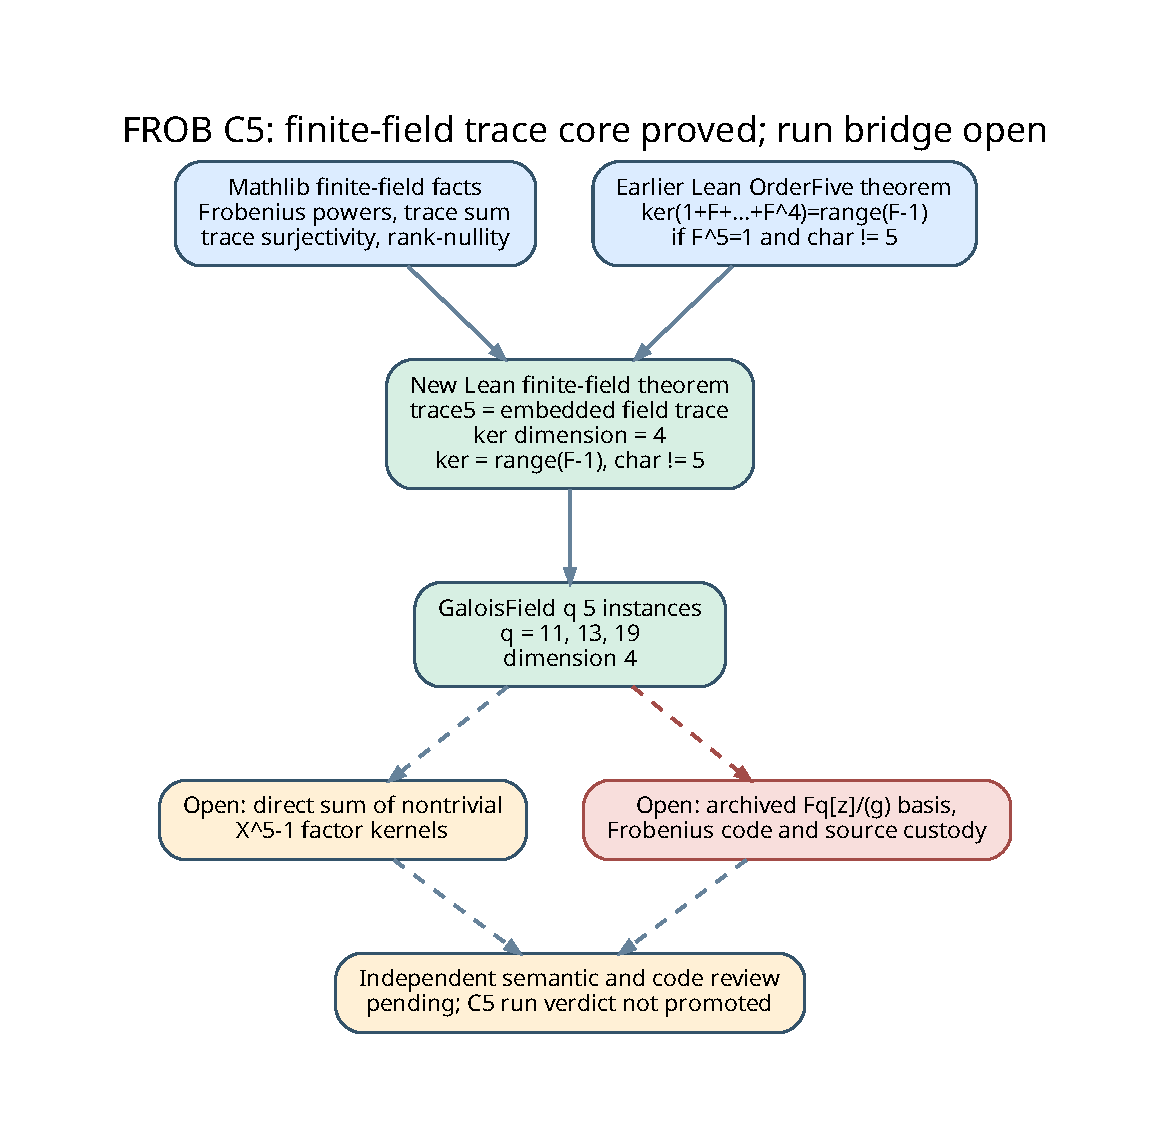
\includegraphics[height=0.82\textheight]{proof-figure.pdf}
\end{center}
\end{document}
